\documentclass{standalone}
\usepackage{tikz}
\usetikzlibrary{patterns, positioning}
\usepackage[sfdefault]{ClearSans} %% option 'sfdefault' activates Clear Sans as the default text font
\usepackage[T1]{fontenc}

\begin{document}
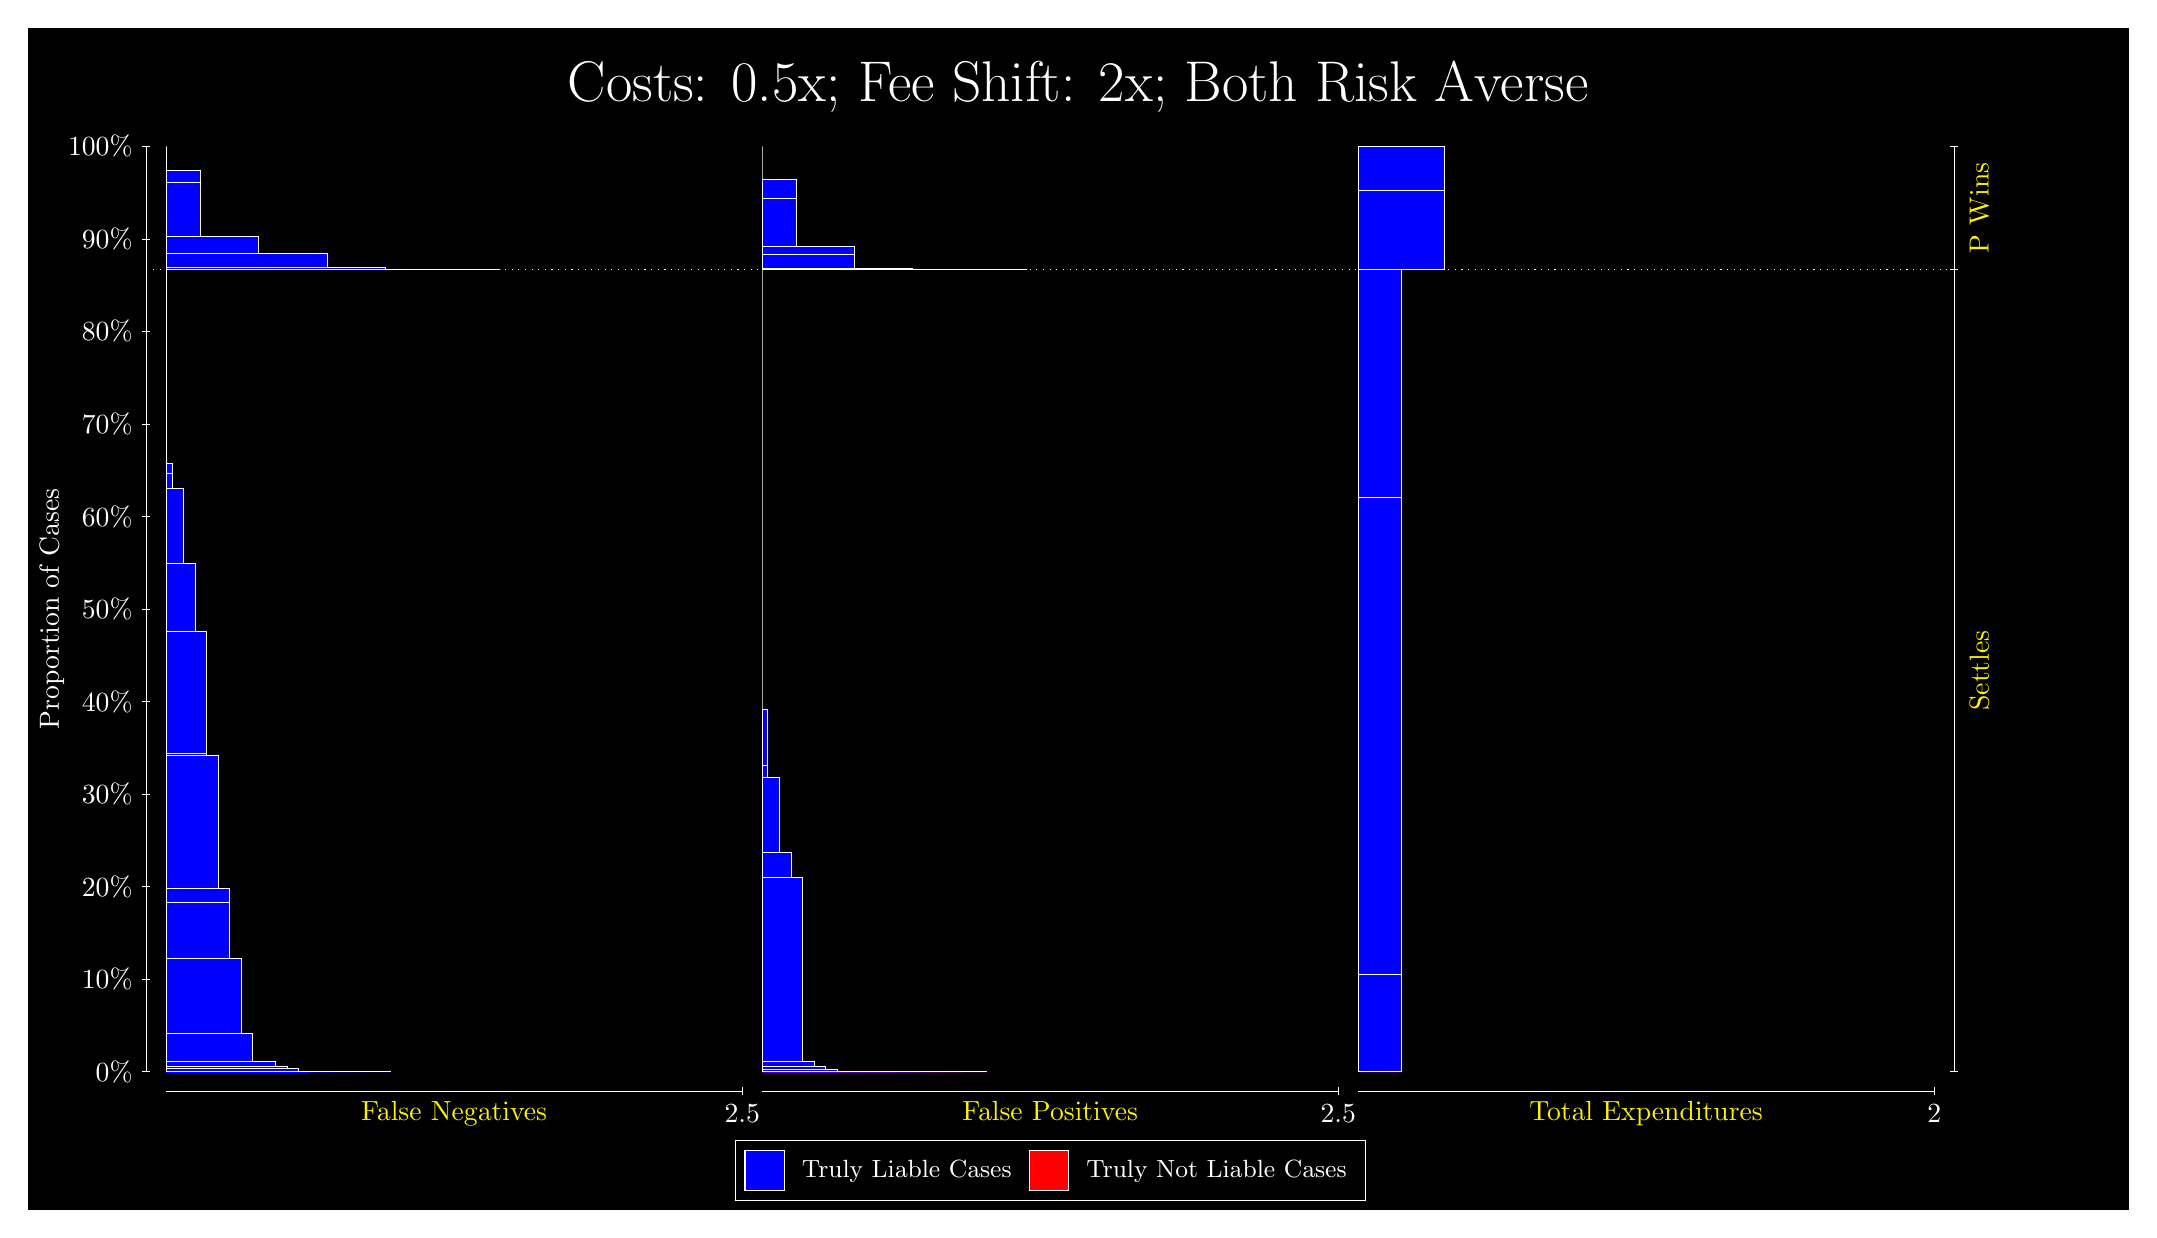
\begin{tikzpicture}
\draw[fill=black] (0,0) rectangle (26.667,15);
\draw[text=white] (0,13.5) rectangle (26.667,15) node[midway] {\huge Costs: 0.5x; Fee Shift: 2x; Both Risk Averse};
\draw[white, very thin] (1.5,1.75) -- (1.5,13.5);
\node[rotate=90, text=white, anchor=center] at (0.3, 7.625) {Proportion of Cases};
\draw[white, very thin] (1.45,1.75) -- (1.55,1.75);
\node[text=white, anchor=east] at (1.45, 1.75) {0\%};
\draw[white, very thin] (1.45,2.925) -- (1.55,2.925);
\node[text=white, anchor=east] at (1.45, 2.925) {10\%};
\draw[white, very thin] (1.45,4.1) -- (1.55,4.1);
\node[text=white, anchor=east] at (1.45, 4.1) {20\%};
\draw[white, very thin] (1.45,5.275) -- (1.55,5.275);
\node[text=white, anchor=east] at (1.45, 5.275) {30\%};
\draw[white, very thin] (1.45,6.45) -- (1.55,6.45);
\node[text=white, anchor=east] at (1.45, 6.45) {40\%};
\draw[white, very thin] (1.45,7.625) -- (1.55,7.625);
\node[text=white, anchor=east] at (1.45, 7.625) {50\%};
\draw[white, very thin] (1.45,8.8) -- (1.55,8.8);
\node[text=white, anchor=east] at (1.45, 8.8) {60\%};
\draw[white, very thin] (1.45,9.975) -- (1.55,9.975);
\node[text=white, anchor=east] at (1.45, 9.975) {70\%};
\draw[white, very thin] (1.45,11.15) -- (1.55,11.15);
\node[text=white, anchor=east] at (1.45, 11.15) {80\%};
\draw[white, very thin] (1.45,12.325) -- (1.55,12.325);
\node[text=white, anchor=east] at (1.45, 12.325) {90\%};
\draw[white, very thin] (1.45,13.5) -- (1.55,13.5);
\node[text=white, anchor=east] at (1.45, 13.5) {100\%};

\draw[white, very thin] (24.457,1.75) -- (24.457,13.5);
\draw[white, very thin] (24.407,1.75) -- (24.507,1.75);
\node[anchor=west] at (24.407, 1.75) {};
\draw[white, very thin] (24.407,11.938) -- (24.507,11.938);
\node[anchor=west] at (24.407, 11.938) {};
\draw[white, very thin] (24.407,13.5) -- (24.507,13.5);
\node[anchor=west] at (24.407, 13.5) {};

\draw[white, very thin, fill=blue] (1.75,1.75) rectangle (4.6044,1.75);
\draw[white, very thin, fill=blue] (1.75,1.75) rectangle (4.3116,1.75);
\draw[white, very thin, fill=blue] (1.75,1.75) rectangle (4.0188,1.75);
\draw[white, very thin, fill=blue] (1.75,1.75) rectangle (3.8725,1.75);
\draw[white, very thin, fill=blue] (1.75,1.75) rectangle (3.7261,1.75);
\draw[white, very thin, fill=blue] (1.75,1.75) rectangle (3.5797,1.7503);
\draw[white, very thin, fill=blue] (1.75,1.7503) rectangle (3.4333,1.7924);
\draw[white, very thin, fill=blue] (1.75,1.7924) rectangle (3.287,1.8229);
\draw[white, very thin, fill=blue] (1.75,1.8229) rectangle (3.1406,1.8836);
\draw[white, very thin, fill=blue] (1.75,1.8836) rectangle (2.9942,1.8847);
\draw[white, very thin, fill=blue] (1.75,1.8847) rectangle (2.8478,2.2328);
\draw[white, very thin, fill=blue] (1.75,2.2328) rectangle (2.7015,3.1911);
\draw[white, very thin, fill=blue] (1.75,3.1911) rectangle (2.5551,3.8954);
\draw[white, very thin, fill=blue] (1.75,3.8954) rectangle (2.5551,4.0736);
\draw[white, very thin, fill=blue] (1.75,4.0736) rectangle (2.4087,5.7654);
\draw[white, very thin, fill=blue] (1.75,5.7654) rectangle (2.2623,5.7948);
\draw[white, very thin, fill=blue] (1.75,5.7948) rectangle (2.2623,7.342);
\draw[white, very thin, fill=blue] (1.75,7.342) rectangle (2.1159,8.2025);
\draw[white, very thin, fill=blue] (1.75,8.2025) rectangle (1.9696,9.1582);
\draw[white, very thin, fill=blue] (1.75,9.1582) rectangle (1.8232,9.3444);
\draw[white, very thin, fill=blue] (1.75,9.3444) rectangle (1.8232,9.4709);
\draw[white, very thin, fill=red] (1.75,9.4709) rectangle (1.75,9.4709);
\draw[white, very thin, fill=blue] (1.75,9.4709) rectangle (1.75,11.938);
\draw[white, very thin, fill=blue] (1.75,11.938) rectangle (5.9949,11.938);
\draw[white, very thin, fill=blue] (1.75,11.938) rectangle (5.2631,11.939);
\draw[white, very thin, fill=blue] (1.75,11.939) rectangle (4.5312,11.969);
\draw[white, very thin, fill=blue] (1.75,11.969) rectangle (4.3848,11.969);
\draw[white, very thin, fill=blue] (1.75,11.969) rectangle (3.7993,12.139);
\draw[white, very thin, fill=blue] (1.75,12.139) rectangle (3.6529,12.139);
\draw[white, very thin, fill=blue] (1.75,12.139) rectangle (3.0674,12.143);
\draw[white, very thin, fill=blue] (1.75,12.143) rectangle (2.921,12.363);
\draw[white, very thin, fill=blue] (1.75,12.363) rectangle (2.3355,12.363);
\draw[white, very thin, fill=blue] (1.75,12.363) rectangle (2.1891,13.043);
\draw[white, very thin, fill=blue] (1.75,13.043) rectangle (2.1891,13.202);
\draw[white, very thin, fill=red] (1.75,13.202) rectangle (1.75,13.202);
\draw[white, very thin, fill=blue] (1.75,13.202) rectangle (1.75,13.5);
\draw[white, very thin, fill=red] (9.3189,1.75) rectangle (12.173,1.75);
\draw[white, very thin, fill=blue] (9.3189,1.75) rectangle (12.173,1.75);
\draw[white, very thin, fill=red] (9.3189,1.75) rectangle (11.88,1.75);
\draw[white, very thin, fill=blue] (9.3189,1.75) rectangle (11.88,1.75);
\draw[white, very thin, fill=red] (9.3189,1.75) rectangle (11.588,1.75);
\draw[white, very thin, fill=blue] (9.3189,1.75) rectangle (11.588,1.75);
\draw[white, very thin, fill=blue] (9.3189,1.75) rectangle (11.441,1.75);
\draw[white, very thin, fill=red] (9.3189,1.75) rectangle (11.295,1.75);
\draw[white, very thin, fill=blue] (9.3189,1.75) rectangle (11.295,1.75);
\draw[white, very thin, fill=blue] (9.3189,1.75) rectangle (11.149,1.75);
\draw[white, very thin, fill=red] (9.3189,1.75) rectangle (11.002,1.75);
\draw[white, very thin, fill=blue] (9.3189,1.75) rectangle (11.002,1.75);
\draw[white, very thin, fill=blue] (9.3189,1.75) rectangle (10.856,1.75);
\draw[white, very thin, fill=red] (9.3189,1.75) rectangle (10.709,1.75);
\draw[white, very thin, fill=blue] (9.3189,1.75) rectangle (10.709,1.75);
\draw[white, very thin, fill=blue] (9.3189,1.75) rectangle (10.563,1.75);
\draw[white, very thin, fill=red] (9.3189,1.75) rectangle (10.417,1.75);
\draw[white, very thin, fill=blue] (9.3189,1.75) rectangle (10.417,1.7521);
\draw[white, very thin, fill=blue] (9.3189,1.7521) rectangle (10.27,1.7821);
\draw[white, very thin, fill=red] (9.3189,1.7821) rectangle (10.124,1.7821);
\draw[white, very thin, fill=blue] (9.3189,1.7821) rectangle (10.124,1.7839);
\draw[white, very thin, fill=blue] (9.3189,1.7839) rectangle (10.124,1.8143);
\draw[white, very thin, fill=blue] (9.3189,1.8143) rectangle (9.9776,1.874);
\draw[white, very thin, fill=red] (9.3189,1.874) rectangle (9.8312,1.874);
\draw[white, very thin, fill=blue] (9.3189,1.874) rectangle (9.8312,4.2165);
\draw[white, very thin, fill=blue] (9.3189,4.2165) rectangle (9.8312,4.2175);
\draw[white, very thin, fill=blue] (9.3189,4.2175) rectangle (9.6848,4.5302);
\draw[white, very thin, fill=blue] (9.3189,4.5302) rectangle (9.5384,5.486);
\draw[white, very thin, fill=blue] (9.3189,5.486) rectangle (9.3921,5.6417);
\draw[white, very thin, fill=blue] (9.3189,5.6417) rectangle (9.3921,6.3465);
\draw[white, very thin, fill=blue] (9.3189,6.3465) rectangle (9.3189,11.938);
\draw[white, very thin, fill=red] (9.3189,11.938) rectangle (12.686,11.938);
\draw[white, very thin, fill=blue] (9.3189,11.938) rectangle (12.686,11.938);
\draw[white, very thin, fill=red] (9.3189,11.938) rectangle (11.954,11.938);
\draw[white, very thin, fill=blue] (9.3189,11.938) rectangle (11.954,11.938);
\draw[white, very thin, fill=blue] (9.3189,11.938) rectangle (11.954,11.939);
\draw[white, very thin, fill=red] (9.3189,11.939) rectangle (11.222,11.939);
\draw[white, very thin, fill=blue] (9.3189,11.939) rectangle (11.222,11.946);
\draw[white, very thin, fill=blue] (9.3189,11.946) rectangle (11.222,11.956);
\draw[white, very thin, fill=red] (9.3189,11.956) rectangle (10.49,11.956);
\draw[white, very thin, fill=blue] (9.3189,11.956) rectangle (10.49,12.133);
\draw[white, very thin, fill=blue] (9.3189,12.133) rectangle (10.49,12.236);
\draw[white, very thin, fill=red] (9.3189,12.236) rectangle (10.344,12.236);
\draw[white, very thin, fill=blue] (9.3189,12.236) rectangle (10.344,12.236);
\draw[white, very thin, fill=blue] (9.3189,12.236) rectangle (9.758,12.837);
\draw[white, very thin, fill=blue] (9.3189,12.837) rectangle (9.758,13.076);
\draw[white, very thin, fill=red] (9.3189,13.076) rectangle (9.6116,13.076);
\draw[white, very thin, fill=blue] (9.3189,13.076) rectangle (9.6116,13.076);
\draw[white, very thin, fill=blue] (9.3189,13.076) rectangle (9.6116,13.076);
\draw[white, very thin, fill=red] (9.3189,13.076) rectangle (9.3189,13.076);
\draw[white, very thin, fill=blue] (9.3189,13.076) rectangle (9.3189,13.5);
\draw[white, very thin, fill=red] (16.888,1.75) rectangle (17.437,1.75);
\draw[white, very thin, fill=blue] (16.888,1.75) rectangle (17.437,2.9896);
\draw[white, very thin, fill=red] (16.888,2.9896) rectangle (17.437,2.9896);
\draw[white, very thin, fill=blue] (16.888,2.9896) rectangle (17.437,9.04);
\draw[white, very thin, fill=red] (16.888,9.04) rectangle (17.437,9.04);
\draw[white, very thin, fill=blue] (16.888,9.04) rectangle (17.437,11.938);
\draw[white, very thin, fill=red] (16.888,11.938) rectangle (17.986,11.938);
\draw[white, very thin, fill=blue] (16.888,11.938) rectangle (17.986,12.944);
\draw[white, very thin, fill=red] (16.888,12.944) rectangle (17.986,12.944);
\draw[white, very thin, fill=blue] (16.888,12.944) rectangle (17.986,13.5);
\draw[white, dotted] (1.5,11.938) -- (24.457,11.938);
\draw[white, very thin] (1.75,1.5) -- (9.0689,1.5);
\node[text=yellow, anchor=north] at (5.4094, 1.5) {False Negatives};
\draw[white, very thin] (9.0689,1.45) -- (9.0689,1.55);
\node[text=white, anchor=north] at (9.0689, 1.45) {2.5};

\draw[white, very thin] (9.3189,1.5) -- (16.638,1.5);
\node[text=yellow, anchor=north] at (12.978, 1.5) {False Positives};
\draw[white, very thin] (16.638,1.45) -- (16.638,1.55);
\node[text=white, anchor=north] at (16.638, 1.45) {2.5};

\draw[white, very thin] (16.888,1.5) -- (24.207,1.5);
\node[text=yellow, anchor=north] at (20.547, 1.5) {Total Expenditures};
\draw[white, very thin] (24.207,1.45) -- (24.207,1.55);
\node[text=white, anchor=north] at (24.207, 1.45) {2};

\node[text=yellow, centered, rotate=90] at (24.777, 6.8442) {Settles};
\node[text=yellow, centered, rotate=90] at (24.777, 12.719) {P Wins};

\draw (12.978300999999998,1.5) node[draw=none] (baseCoordinate) {};
\begin{scope}[align=center]
        \matrix[scale=0.5, draw=white, below=0.5cm of baseCoordinate, nodes={draw}, column sep=0.1cm]{
            \node[rectangle, draw, minimum width=0.5cm, minimum height=0.5cm, fill=blue] {}; &
            \node[draw=none, font=\small, text=white] (B) {Truly Liable Cases}; &
            \node[rectangle, draw, minimum width=0.5cm, minimum height=0.5cm, fill=red] {}; &
            \node[draw=none, font=\small, text=white] (B) {Truly Not Liable Cases}; \\
            };
\end{scope}

\end{tikzpicture}
\end{document}